\section{Technische bijlage Proof of Concept}
\label{technische-bijlage}
\subsection{Functie voor opbouw vectorstore}
\label{functie-vectorstore}

\begin{lstlisting}[basicstyle=\small, frame=single, breaklines=true, postbreak=\mbox{\textcolor{red}{$\hookrightarrow$}\space}, escapeinside ={\%,}, escapechar={!},
    numbers=left, language=Python, caption=Aanmaken van de vectorstore]
def build_vector_store(embeddings_function, document_path, db_name, search_type, search_kwargs):
    base_dir = os.path.abspath(os.path.join(os.path.dirname(__file__), "../../resources"))
    persistent_directory = os.path.join(base_dir, "vector_db", db_name)
    loader_mapping = {
        ".md": TextLoader,
        ".txt": TextLoader,
        ".pdf": PyPDFLoader,
        ".docx": UnstructuredWordDocumentLoader,
        ".doc": UnstructuredWordDocumentLoader,
    }
    
    # Check if the Chroma vector store already exists
    print("Persistent directory does not exist. Initializing vector store...")
    
    documents = []
    # Iterate over each folder in the path
    for folder in glob.glob(f"{document_path}/*"):
        if os.path.isdir(folder):
            # Iterate over each file in the folder
            for ext, base_loader_type in loader_mapping.items():
                for doc_file_path in glob.glob(os.path.join(folder, f"*{ext}")):
                    try:
                        # Use the appropriate loader based on the file extension
                        document = base_loader_type(doc_file_path, encoding="utf-8")
                        doc = document.load()
                        for d in doc:
                            d.metadata = {"source": doc_file_path, "folder": folder}
                            documents.append(d)
                    except Exception as e:
                        print(f"Failed to load file {doc_file_path}: {e}")
        
    # Split the document into chunks
    text_splitter = RecursiveCharacterTextSplitter(chunk_size=2000, chunk_overlap=500)
    docs = text_splitter.split_documents(documents)
    
    # Display information about the split documents
    print("\n--- Document Chunks Information ---")
    print(f"Number of document chunks: {len(docs)}")
    
    # Create the vector store and persist it automatically
    print("\n--- Creating vector store ---")
    
    # Return a ChromaDB instance
    return (Chroma.from_documents(
        docs, embeddings_function, persist_directory=persistent_directory)
        .as_retriever(search_type=search_type, search_kwargs=search_kwargs)
        )
\end{lstlisting}

\subsection{Chunks in verschillende formaten}
\label{chunks-verschillende-formaten}
\subsubsection{PDF}
\begin{figure}[H]
    \centering
    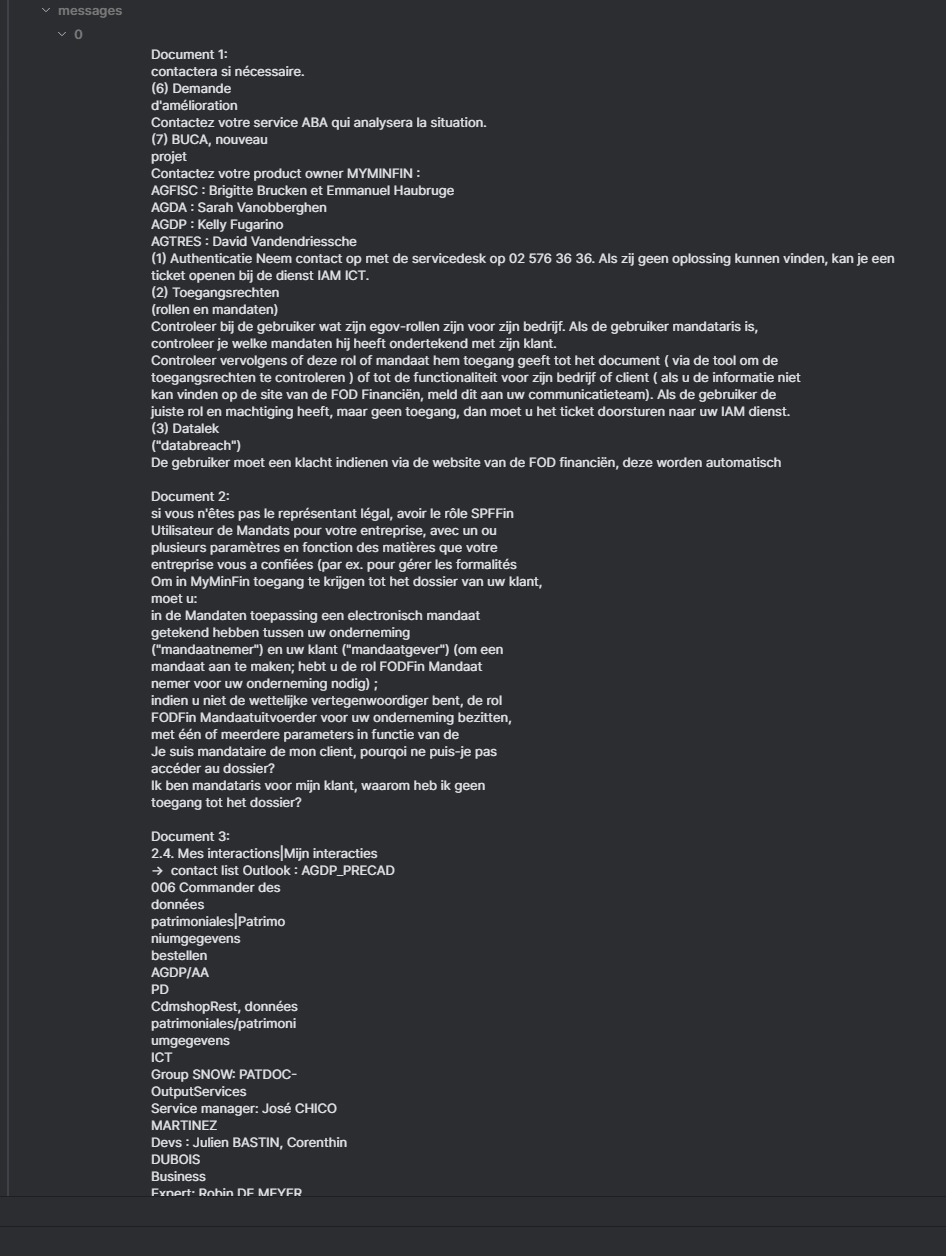
\includegraphics[width=\linewidth]{chunks_pdf.png}
    \caption{Opgehaalde chunks in PDF}
    \label{fig:chunks_pdf}
\end{figure}

\subsubsection{Docx}
\begin{figure}[H]
   \centering
   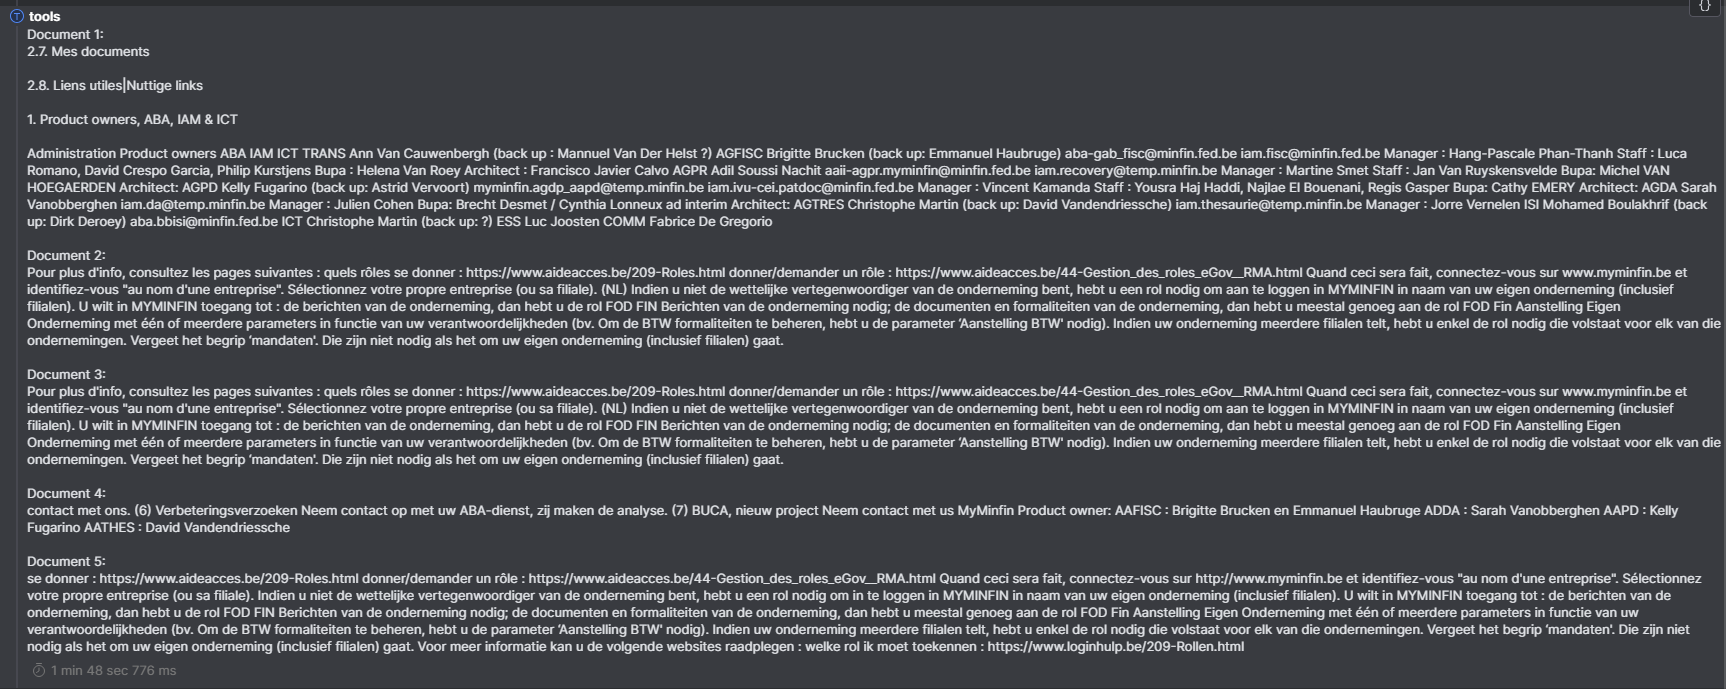
\includegraphics[width=\linewidth]{chunks_docx.png}
   \caption{Opgehaalde chunks in DOCX}
   \label{fig:chunks_doc}
\end{figure}


\subsubsection{Markdown}
\begin{figure}[H]
    \centering
    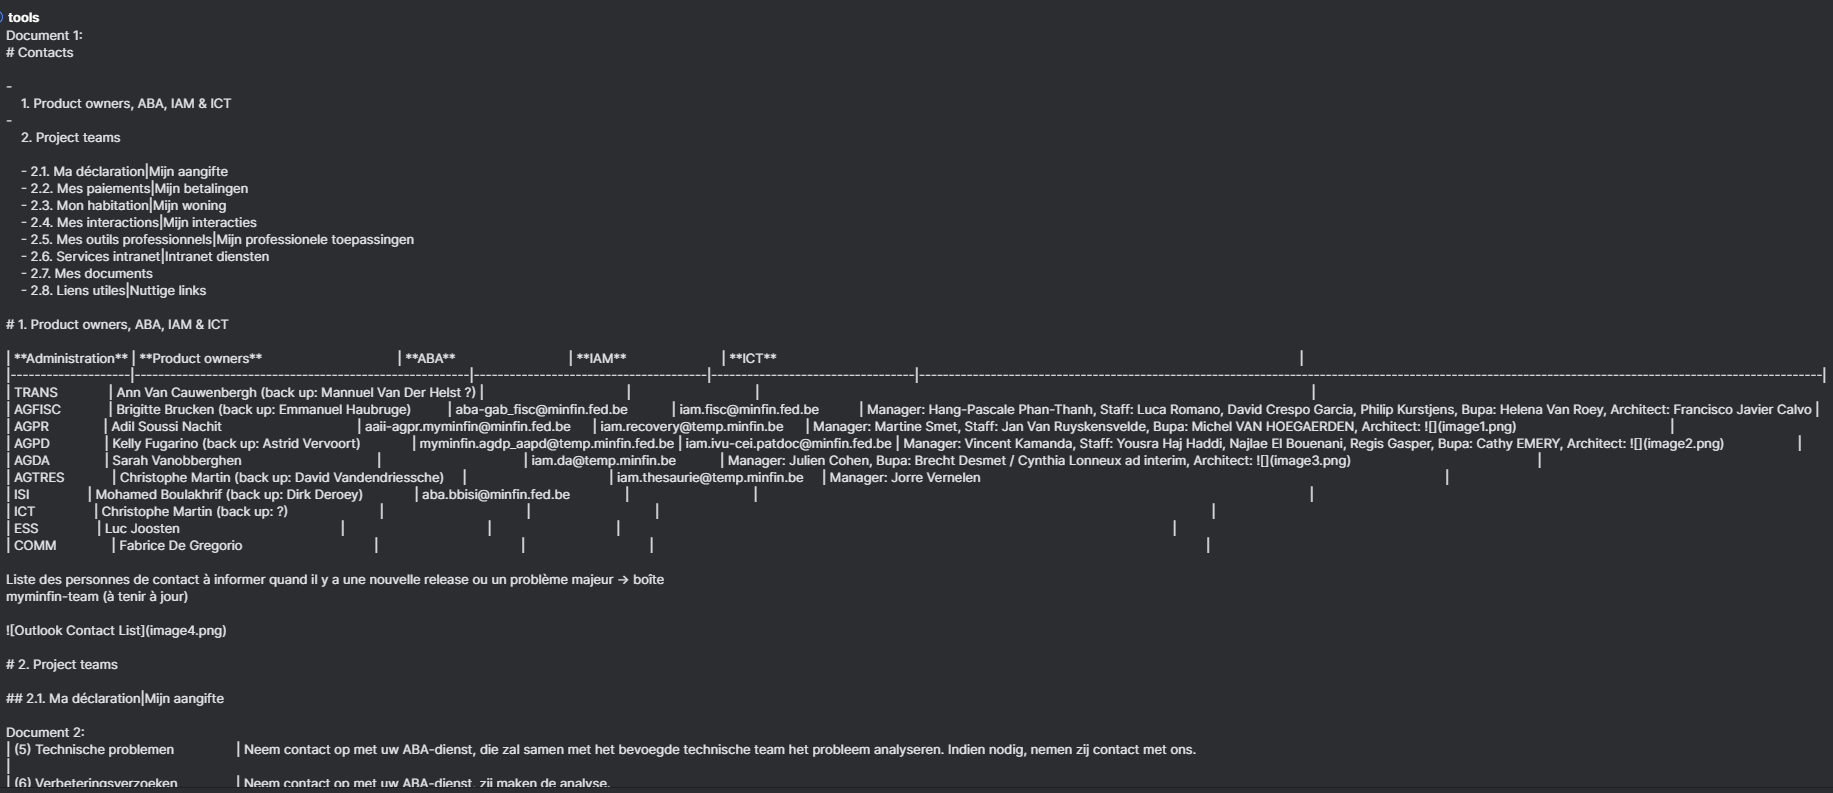
\includegraphics[width=\linewidth]{chunks_md.png}
    \caption{Opgehaalde chunks in Markdown}
    \label{fig:chunks_md}
\end{figure}

